\documentclass[11pt]{article}
%% Package imports
\usepackage[utf8]{inputenc}
\usepackage{amsmath}
\usepackage{subcaption}
\usepackage{amsfonts}
\usepackage{amssymb}
\usepackage{physics}
\usepackage{graphicx}
\usepackage[left=1cm,right=1cm,top=2cm,bottom=2cm]{geometry}
\usepackage{multirow}
\usepackage{booktabs}
\usepackage{float}
\usepackage{verbatim}
\usepackage{amsthm}
\usepackage{minted}
\usepackage{fancyhdr}
\usepackage{subcaption}
\usepackage[dvipsnames]{xcolor}
\usepackage{parskip}
\usepackage{blindtext}
\usepackage{hyperref}
\usepackage{listings,xcolor}
\usepackage[T1]{fontenc}
\usepackage{xcolor}
\usepackage[scaled=0.9]{DejaVuSansMono}
\definecolor{commentgreen}{RGB}{2,112,10}
\definecolor{eminence}{RGB}{108,48,130}
\definecolor{weborange}{RGB}{255,165,0}
\definecolor{frenchplum}{RGB}{129,20,83}

\lstdefinelanguage{elixir}{
    morekeywords={case,catch,def,do,else,false,%
        use,alias,receive,timeout,defmacro,defp,%
        for,if,import,defmodule,defprotocol,%
        nil,defmacrop,defoverridable,defimpl,%
        super,fn,raise,true,try,end,with,%
        unless},
    otherkeywords={<-,->, |>, \%\{, \}, \{, \, (, )},
    sensitive=true,
    morecomment=[l]{\#},
    morecomment=[n]{/*}{*/},
    morecomment=[s][\color{purple}]{:}{\ },
    morestring=[s][\color{orange}]"",
    commentstyle=\color{commentgreen},
    keywordstyle=\color{eminence},
    stringstyle=\color{red},
	basicstyle=\ttfamily,
	breaklines,
	showstringspaces=false,
	frame=tb
}

\lstset{numbers=left,xleftmargin=2em,frame=single,framexleftmargin=0em,numberstyle=\footnotesize\ttfamily}
\renewcommand{\baselinestretch}{1.5}

%% Commands for inserting big braces.
\newcommand\lb{\left\lbrace}
\newcommand\rb{\right\rbrace}

%% Math symbols
\usepackage[shortlabels]{enumitem}
\usepackage{titling}
\setlength{\droptitle}{-3cm}

%% Page style settings
\pagestyle{fancy}
\fancyfoot{}
\fancyhead[L]{\slshape{Multi-Paxos}}
\fancyhead[R]{\slshape{Szymon Kubica, CID: 01871147}}
\fancyfoot[C]{\thepage}
\begin{document}

\title{Distributed Algorithms 60009 \ Coursework - Multi-Paxos}
\date{\today}
\author{Szymon Kubica, (sk4520) CID: 01871147}
 {\let\newpage\relax\maketitle}

\section*{Architecture}
At the top level of the system the Multipaxos module spawns a collection of
Servers and Clients and the Monitor which keeps track of the state of the whole
system. Each Server has its own Database, Replica, Leader and Acceptor. The
initial binding of the modules is done by Multipaxos, each replica gets bound
to all leaders and each leader gets bound to all acceptors and replicas,
each client gets access to all replicas. I omitted the corresponding \texttt{:BIND}
messages.
\begin{figure}[H]
    \centering
    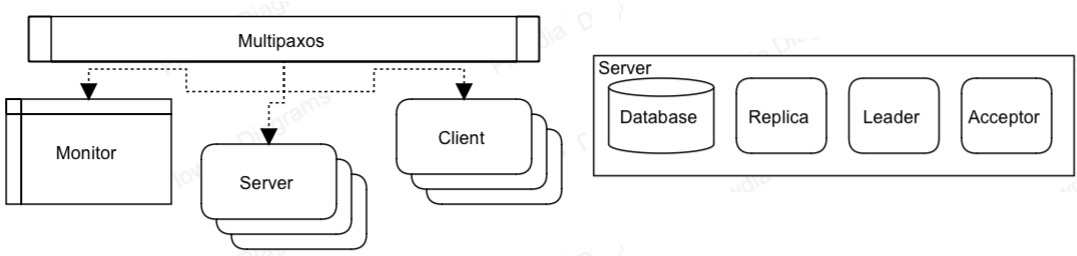
\includegraphics[width=400px]{architecture0.png}
    \caption{Top-level architecture.}
    \vspace{-15pt}
\end{figure}
A typical client request flow can be seen in Figure 2 below. The dotted arrows
represent spawned child processes, the black solid ones represent directed messages
with one recipient, whereas the blue ones represent messages which are broadcast
to all modules of a given type. Diagram on the left depicts the phase 1 of the synod protocol,
whereas phase 2 can be seen on the right. On the left one of the scouts
got preempted and one got adopted. On the right a commander got accepted
and broadcast its decision to all replicas which have
sent execute requests to the databases.
    \vspace{-5pt}
\begin{figure}[H]
    \centering
    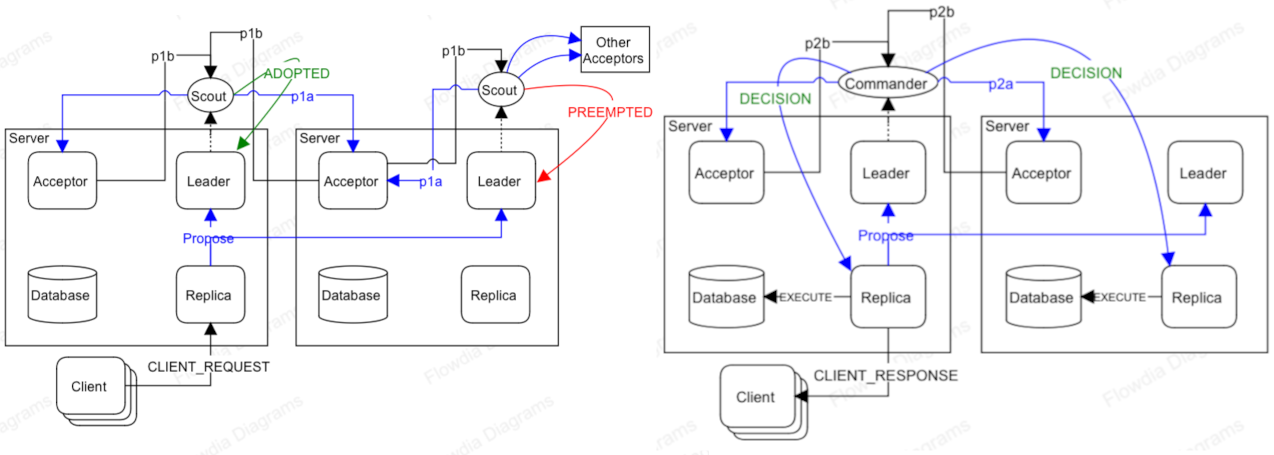
\includegraphics[width=\textwidth]{architecture1.png}
    \caption{Typical client request flow.}
\end{figure}

\pagebreak
\section*{Liveness}
My initial implementation of the section 3 followed closely the algorithm
described in the paper. Each leader after receiving a \texttt{:PREEMPTED}
message becomes inactive and starts pinging the leader that has preempted it,
instead of picking a higher ballot number and spawning a scout immediately. I
implemented that by spawning one failure detector module for each leader. When
preempted, a leader notifies its failure detector, which starts pinging the
leader associated with the preempting ballot \texttt{b}, then the leader
deactivates itself and continues.
\begin{lstlisting}[language=elixir, caption={New way of handling \texttt{:PREEMPTED} messages.},captionpos=b]
{:PREEMPTED, b} ->
  send(self.failure_detector, {:PING, b})
  self |> deactivate |> next
\end{lstlisting}
Each leader associates a timeout with its current ballot number. Every time a
leader gets preempted, its next ballot will use a longer timeout (multiplicative
increase). However, the timeout of the current ballot decreases linearly with each
proposal chosen for that ballot. It is done by sending an appropriate notification
from the commander after a \texttt{:DECISION} message is sent to the replicas.
Whenever an active leader gets pinged by FD of some other leader, it sends
its timeout back, and the FD updates it and uses it from now on.
\begin{lstlisting}[language=elixir, caption={Leader responding to a ping message.},captionpos=b]
{:RESPONSE_REQUESTED, requestor} ->
    cond do
      self.active -> send(requestor, {:STILL_ALIVE, ballot_num, timeout})
      self.preempted_by != nil -> send(requestor, {:STILL_ALIVE, preempted_by, timeout})
\end{lstlisting}
When tweaking the timeout settings, it was very difficult to pick the
appropriate constants. If the timeout decreased too quickly or it didn't grow
enough after preemptions, all leaders ended up preempting each other which
impacted performance. I noticed that we don't prioritise fairness, it is
perfectly fine if one leader is working on its ballot and all of the other ones
keep pinging it regularly and only react if they detect a failure. I added a
new version of the failure detector which has a static timeout. I realised that
it could happen that three leaders $\lambda_1$, $\lambda_2$,  $\lambda_3$
behave as follows: $\lambda_2$ preempts $\lambda_1$ and $\lambda_3$ preempts
$\lambda_2$, in which case $\lambda_2$ becomes inactive and stops responding to
$\lambda_1$'s pings, thus $\lambda_1$ wakes up and can possibly preempt
$\lambda_3$. Even though variable timeouts would help to solve this issue and
prevent it from live-locking, it introduces an unnecessary congestion. I solved
this problem by having each leader record the last preempting ballot number. If
a leader was recently preempted and is now inactive and gets pinged by somebody
whom he preempted before, it sends the ballot number that preempted it back to
the requestor (Listing 2 above). That way the leader who pinged us doesn't wake up immediately
but starts pinging the leader who is currently working.
\pagebreak
\section*{Evaluation}
\subsection*{Hardware}
The evaluation was conducted on my laptop with the following specification:

OS: Linux 6.1.12-arch1-1, processor: 11th Gen Intel i7-1165G7 4.700GHz, cores: 8, ram: 32GB.

\subsection*{Live-locking Implementation and a Partial Fix}
After implementing the multi-paxos without liveness as described in the paper,
I found that the system would live-lock even with 5 requests per client (there
was 5 clients so it amounts to 25 requests total). To solve the issue for small
numbers of requests, I decided to have each leader sleep for a random period of
time after it gets preempted. I found that for small numbers of requests (see
Figure 3 below) it didn't live-lock, however, when ran with the default config
(5 clients, 5 servers and 500 requests per client in a round-robin setting) the
partial fix to the liveness problem also live-locked. In the figure below on the
right you would normally expect to get to 2500 requests total. The logs corresponding to
those two runs can be found in the files with reference numbers from 01 to 04.
\begin{figure}[H]
    \begin{subfigure}[b]{0.5\textwidth}
    \centering
    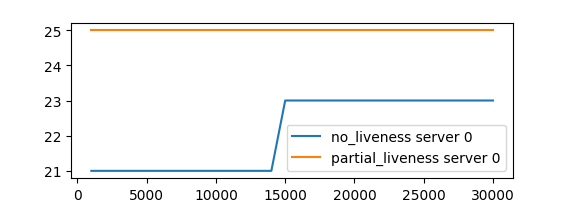
\includegraphics[width=\textwidth]{no_liveness_partial_liveness.png}
  \end{subfigure}%
    \begin{subfigure}[b]{0.5\textwidth}
    \centering
    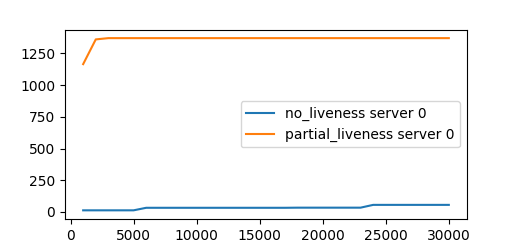
\includegraphics[width=\textwidth]{medium.png}
    \end{subfigure}
    \centering
    \caption{5 servers and 5 clients with 5 and 500 requests respectively.}
    \vspace{-15pt}
\end{figure}
\subsection*{Full Liveness and Simple Liveness}
The most interesting observation that I made when running different configurations
of my implementation for liveness was that the performance of the system was
dependent on the configuration settings for the timeouts. If settings are picked incorrectly,
the leaders can decrease their timeouts too quickly then get preempted immediately.
One big disadvantage of the AIMD-like approach described in the paper was that
a leader who is successful in getting its proposals accepted decreases the timeout
associated with its ballot, and therefore it will eventually get preempted by one
of the leaders who are pinging it. That's not necessarily what we want for performance. I noticed that after preempting a leader it takes a while for the system to make
new decisions because all of the leaders who were previously pinging the main leader have now
sent scouts and are competing against each other for being the first one who preempts
everyone else. It tends to happen that multiple of them get adopted, and the leaders spawn
new commanders. Given that each active leader will spawn one commander for each slot,
when we have 10000 slots, the system gets congested with messages and it takes
a very long time before the acceptors can accept one commander successfully.
That can be seen in the figure below, the log files associated with it have
reference numbers 08, 09, 10.
\begin{figure}[H]
    \centering
    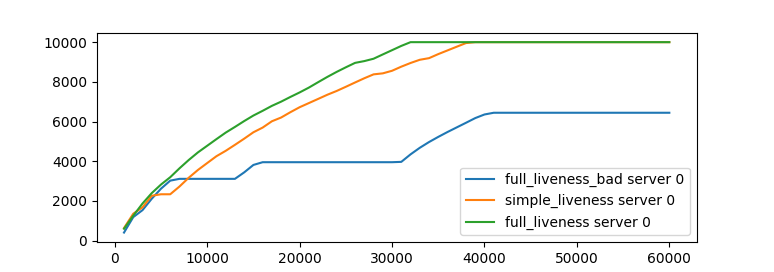
\includegraphics[width=400px]{liveness_simple_bad_config.png}
    \caption{2000 requests with 5 servers and 5 clients.}
    \vspace{-15pt}
\end{figure}
The figure above illustrates the performance of three different configurations.
The one in green is the liveness implementation described in the paper with some
sane bounds imposed on the range of timeouts that can be associated with each ballot.
The one in orange is the simple implementation with a static timeout that I described
in the Liveness section. The one in blue is the liveness implementation where the
timeout changing settings were tuned incorrectly. As you can see it has periods
where it is making progress, however it also has three sections where the system
looks like it is stuck. Before each of those sections what happens is that the current
main leader gets preempted and the others compete against each other to get accepted.
Because their timeouts are adjusted incorrectly, it takes a long time before one of
them finally manages to secure a ballot. This occurs because as the main leader gets
preempted, the others start spawning scouts and it can happen that multiple of them receive
an adopted message and cause the leaders to spawn new commanders, which exerts a high
stress on acceptors and the whole system slows down.

Another interesting observation was that the system seems to get slower over time,
If you examine the Figure 4 above, you can see that the green line representing
the correctly-configured liveness implementation is not straight, its gradient decreases
which means that as the number of accepted requests grows, the system is able to
make less progress in a given time period. A possible cause of this behaviour
is that the acceptors maintain a MapSet of all accepted pvalues, therefore as the
number of accepted proposals approaches 10000, they keep sending those MapSets around
and each leader when updating its pvalues needs to iterate over the big object.

Having conducted these experiments, I have concluded that the most desirable
situation is where one leader gets to preempt everyone else at the beginning, and
then within a single ballot processes all requests while the others are patiently
pinging it to check if it hasn't crashed. If they detect a failure they should
act accordingly and "elect" (by fighting who gets accepted first) and then continue
processing the remaining requests.
\subsection*{Crash Failure Experiments}
To examine failures I have checked if two servers crashing
impact the liveness of the system. In the figure below on the left you can see a run
where two servers crash right at the start of it. The configuration used during that
run was 5 clients, 5 servers and 500 requests per client. I found that, when compared
to Figure 3, two servers crashing allowed the system to perform more requests, although
it still live-locked in the end. That run has reference number 06.
\begin{figure}[H]
          \begin{subfigure}[b]{0.35\textwidth}
      \centering
      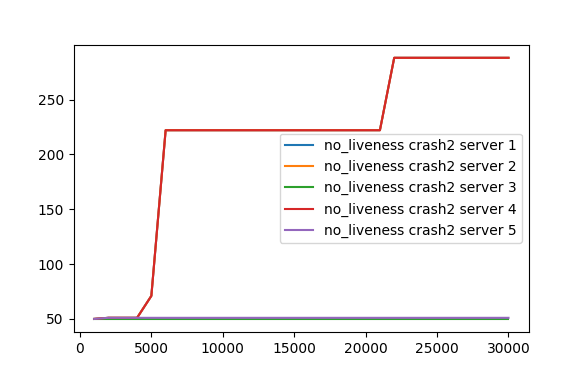
\includegraphics[width=200px]{crash2.png}
      \caption{Crash Failure and Liveness}
    \end{subfigure}%
\begin{subfigure}[b]{0.65\textwidth}
      \centering
      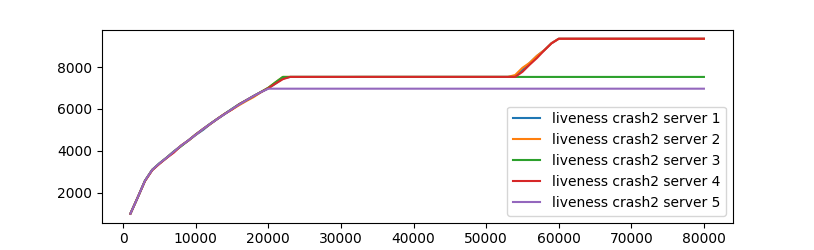
\includegraphics[width=400px]{crash2_liveness.png}
      \caption{Main Leader Crash Failure.}
    \end{subfigure}

    \centering
      \caption{Crash Failure Testing}
    \vspace{-15pt}
\end{figure}
As I explained before the most desirable situation is when a single leader gets
to decide on all proposals. However, the immediate issue that question that
comes up is: Does the system continue to work if that main leader crashes? The
configuration used was the same as in Figure 4, and the server 5 and 3 crashed
after 20 and 22 seconds respectively. The logs can be found in the output file
with reference number 11. I needed to re-run the experiment several times to
make sure that that main leader crashes. In the figure above you can see that
at the start there was a single leader responsible for deciding on all
proposals (because there are no pauses). After leader 3 has crashed, the system
didn't accept any new requests for about 30 seconds. It could look like a live
lock, however after looking at the logs below one can see that the leader who
eventually started processing new commands only needed to
spawn two sets of commanders (roughly 2 times 7000). A live-lock normally causes the system to be
flooded with scouts and many more commanders than we have in this case. This indicates that the
system is able to recover from crash failures.
\begin{lstlisting}[language=elixir, caption={Commanders spawned before starting to make progress.},captionpos=b]
time = 22000  db requests done = [{1, 7454}, {2, 7530}, {3, 7529}, {4, 7422}, {5, 6967}]
time = 22000  commanders up = [{1, 1064}, {2, 0}, {3, 7530}, {4, 0}, {5, 1063}]
time = 22000  commanders down = [{1, 1064}, {2, 0}, {3, 7530}, {4, 0}, {5, 1063}]
...
time = 55000  db requests done = [{1, 7853}, {2, 7965}, {3, 7529}, {4, 7771}, {5, 6967}]
time = 55000  commanders up = [{1, 1064}, {2, 15081}, {3, 7530}, {4, 15514}, {5, 1063}]
time = 55000  commanders down = [{1, 1064}, {2, 15081}, {3, 7530}, {4, 15513}, {5, 1063}]
\end{lstlisting}

\end{document}
